% cv.tex — compile avec XeLaTeX (recommandé) : xelatex cv.tex
\documentclass[11pt,a4paper]{article}

% --------- Packages ----------
\usepackage[a4paper,margin=0mm]{geometry}
\usepackage{graphicx}
\usepackage{tikz}
\usepackage{tabularx}
\usepackage{enumitem}
\usepackage{setspace}
\usepackage{hyperref}
\usepackage{fontspec}
\usepackage{xcolor}

% --------- Fonts (XeLaTeX) ----------
\setmainfont{TeX Gyre Heros} % proche d'Helvetica/Arial
\newfontfamily\TitleFont{TeX Gyre Heros}

% --------- Colors ----------
\definecolor{SidebarBlack}{HTML}{0B0B0B}
\definecolor{AccentYellow}{HTML}{E6C64A}
\definecolor{TextGray}{HTML}{333333}
\definecolor{LightGray}{HTML}{777777}

% --------- Layout constants ----------
\newcommand{\SidebarW}{0.34} % ~1/3
\newcommand{\MainW}{0.66}

\setlength{\parindent}{0pt}
\setlength{\parskip}{0pt}

\hypersetup{
  colorlinks=true,
  urlcolor=TextGray,
  linkcolor=TextGray
}

% --------- Helpers ----------
\newcommand{\SectionTitle}[1]{%
  \vspace{8pt}
  {\TitleFont\bfseries\large\letterspace to 1.5pt{#1}}\par
  \vspace{6pt}
}

\newcommand{\SideTitle}[1]{%
  \vspace{16pt}
  {\TitleFont\bfseries\large\color{white}\letterspace to 1.5pt{#1}}\par
  \vspace{8pt}
}

\newcommand{\SmallWhite}[1]{\color{white}\fontsize{10.3}{12}\selectfont #1}
\newcommand{\SmallGray}[1]{\color{LightGray}\fontsize{10.3}{12}\selectfont #1}
\newcommand{\BodyText}[1]{\color{TextGray}\fontsize{10.6}{13}\selectfont #1}

\newcommand{\XPItem}[4]{%
  % #1 = titre, #2 = date (à droite), #3 = sous-titre, #4 = bullets
  \begin{tabularx}{\linewidth}{@{}X r@{}}
    {\TitleFont\bfseries\BodyText{#1}} & {\TitleFont\bfseries\BodyText{#2}}\\
  \end{tabularx}
  \vspace{2pt}
  {\SmallGray{#3}}\par
  \vspace{6pt}
  \begin{itemize}[leftmargin=14pt,itemsep=3pt,topsep=0pt]
    #4
  \end{itemize}
  \vspace{6pt}
}

\newcommand{\FormationItem}[3]{%
  \begin{tabularx}{\linewidth}{@{}X r@{}}
    {\TitleFont\bfseries\BodyText{#1}} & {\TitleFont\bfseries\BodyText{#2}}\\
  \end{tabularx}
  \vspace{2pt}
  {\SmallGray{#3}}\par
  \vspace{6pt}
}

% --------- Document ----------
\begin{document}
\thispagestyle{empty}

% Full-page background blocks
\begin{tikzpicture}[remember picture,overlay]
  \fill[SidebarBlack] (current page.north west) rectangle
    ([xshift=\SidebarW\paperwidth]current page.south west);
  \fill[white] ([xshift=\SidebarW\paperwidth]current page.north west) rectangle
    (current page.south east);
\end{tikzpicture}

% Content area split
\begin{minipage}[t][\paperheight]{\SidebarW\paperwidth}
  \vspace*{16mm}
  \hspace*{10mm}
  \begin{minipage}[t]{\linewidth-20mm}

    % NAME block
    {\TitleFont\bfseries\fontsize{20}{22}\selectfont\color{white}HERR}\par
    \vspace{2pt}
    {\TitleFont\bfseries\fontsize{18}{20}\selectfont\color{white}Maximilien}\par
    \vspace{6pt}
    {\TitleFont\fontsize{12}{14}\selectfont\color{white}22 ans}\par

    \vspace{14pt}

    % PHOTO (remplace ./photo.jpg)
    \begin{center}
      \begin{tikzpicture}
        \node[inner sep=0pt,draw=AccentYellow,line width=3pt] {\includegraphics[width=0.78\linewidth]{photo.jpg}};
      \end{tikzpicture}
    \end{center}

    % CONTACT
    \SideTitle{CONTACT}
    % Icônes optionnelles: remplace par images si tu veux
    \SmallWhite{\textbf{✉} \href{mailto:maximilienherr@gmail.com}{maximilienherr@gmail.com}}\par
    \vspace{6pt}
    \SmallWhite{\textbf{in} \href{https://www.linkedin.com/in/maximilien-herr}{maximilien-herr}}\par

    % LANGUES
    \SideTitle{LANGUES}
    % Flags optionnels: ajoute des PNG (uk.png, de.png) et décommente
    % \SmallWhite{\includegraphics[height=10pt]{uk.png}\hspace{6pt}Anglais : niveau C1}\par
    % \vspace{6pt}
    % \SmallWhite{\includegraphics[height=10pt]{de.png}\hspace{6pt}Allemand : niveau B1}\par
    \SmallWhite{Anglais : niveau C1}\par
    \vspace{6pt}
    \SmallWhite{Allemand : niveau B1}\par

    % PERSONNALITÉ
    \SideTitle{PERSONNALITÉ}
    \SmallWhite{Résolution de problèmes et sens du détail}\par
    \vspace{6pt}
    \SmallWhite{Structuration de solutions techniques complexes}\par
    \vspace{6pt}
    \SmallWhite{Communication technique claire (écrit/oral)}\par
    \vspace{6pt}
    \SmallWhite{Vision produit orientée impact business}\par

    % INTÉRÊTS
    \SideTitle{INTÉRÊTS}
    \SmallWhite{\textbf{Salons techs internationaux}}\par
    \vspace{4pt}
    \SmallWhite{Depuis que je suis rédacteur, je couvre des salons techs à l’international, comme Vivatech à Paris, l’IFA à Berlin, ou encore la Gamescom à Cologne !}\par

    \vspace{12pt}
    \SmallWhite{\textbf{Judoka à un niveau compétitif}}\par
    \vspace{4pt}
    \SmallWhite{Sport pratiqué pendant plus de 7 ans, qui m’a permis de développer une confiance personnelle, un esprit de rigueur, et les valeurs de ce sport.}\par

  \end{minipage}
\end{minipage}
\begin{minipage}[t][\paperheight]{\MainW\paperwidth}
  \vspace*{16mm}
  \hspace*{12mm}
  \begin{minipage}[t]{\linewidth-24mm}

    % QUOTE (haut de page)
    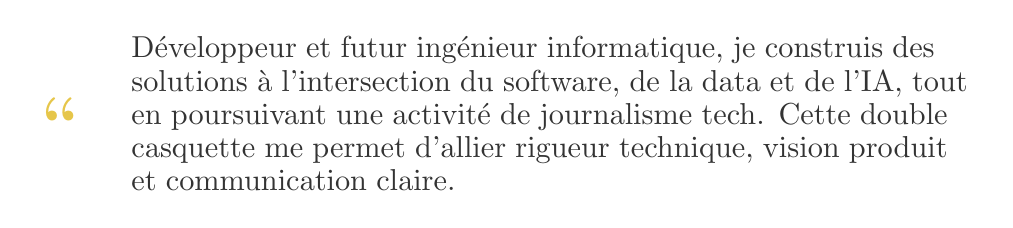
\begin{tikzpicture}
      \node[anchor=west] at (0,0) {\TitleFont\bfseries\fontsize{46}{46}\selectfont\color{AccentYellow}``};
      \node[anchor=west,text width=\linewidth-14mm] at (12mm,1mm) {%
        \BodyText{Développeur et futur ingénieur informatique, je construis des solutions à l’intersection du software, de la data et de l’IA, tout en poursuivant une activité de journalisme tech. Cette double casquette me permet d’allier rigueur technique, vision produit et communication claire.}
      };
    \end{tikzpicture}

    % EXPERIENCES
    \SectionTitle{EXPÉRIENCES}
    \XPItem
      {Ingénieur Big Data \& IA}
      {Depuis septembre 2023}
      {Smartfluence - AI Global Influence}
      {
        \item \BodyText{Architecture technique orientée data/IA (Django, PostgreSQL, Redis, S3) et pipelines de traitement.}
        \item \BodyText{Développement d’un outil d’analyse/agrégation de données sociales à grande échelle (+2M profils).}
        \item \BodyText{Mise en place CI/CD, monitoring des services et livraison rapide de sites marketing.}
      }

    \XPItem
      {Stagiaire Ingénieur Informatique}
      {Juin 2025 à août 2025}
      {ITMI, Sept-Îles (Québec, Canada)}
      {
        \item \BodyText{Stage international de 3 mois en environnement industriel.}
        \item \BodyText{Collaboration avec les équipes locales sur des sujets d’ingénierie informatique.}
      }

    \XPItem
      {Journaliste Tech Freelance}
      {Depuis août 2020}
      {Frandroid, Le Café du Geek, DroidSoft, ex-Clubic}
      {
        \item \BodyText{Rédaction de tests, actualités et dossiers techniques.}
        \item \BodyText{Couverture de salons tech internationaux.}
        \item \BodyText{SEO, HTML/CSS et vulgarisation de sujets IA.}
      }

    \XPItem
      {Développeur Web}
      {Avril 2023 à juin 2023}
      {Agence Geek Media - développement d’outils pour DroidSoft}
      {
        \item \BodyText{Création d’un comparateur de smartphones, tablettes et montres.}
        \item \BodyText{Plugins WordPress en PHP, backend/frontend/API et scripts d’alimentation de base de données.}
      }

    % FORMATION
    \SectionTitle{FORMATION}
    \FormationItem
      {Diplôme d’ingénieur Informatique}
      {Septembre 2023 à août 2026}
      {Ecole d’ingénieur de l’ISIMA, Clermont-Ferrand (63)}

    \FormationItem
      {BUT Informatique Graphique}
      {Septembre 2021 à juin 2023}
      {IUT Informatique Graphique de l'UCA, Puy-en-Velay (43)}

    \FormationItem
      {Baccalauréat Scientifique Mention TB}
      {Septembre 2018 à juin 2021}
      {Lycée de Saint-Julien, Brioude (43). Spécialités mathématiques (options mathématiques expertes), physique-chimie, histoire, géographie, géopolitique et science politique.}

    % COMPETENCES
    \SectionTitle{COMPÉTENCES}
    \BodyText{\textbf{Langages de programmation :} Python, TypeScript/JavaScript, C++, C, C\#}\par
    \vspace{4pt}
    \BodyText{\textbf{Data \& IA :} Machine Learning, Deep Learning, IA générative, RL (Q-Learning, DQN, PPO, SAC)}\par
    \vspace{4pt}
    \BodyText{\textbf{Web \& backend :} Django, Node.js/Express, Next.js, HTML/CSS, PHP}\par
    \vspace{4pt}
    \BodyText{\textbf{Data stores \& DevOps :} PostgreSQL, MySQL, Redis, MongoDB, Docker, CI/CD, monitoring}\par
    \vspace{4pt}
    \BodyText{Communication technique, rédaction web, SEO et anglais professionnel}\par
    \vspace{6pt}
    \SmallGray{Références et projets détaillés disponibles sur demande.}\par

  \end{minipage}
\end{minipage}

\end{document}
